
%==============================================================================

\section{Theoretical background}
\subsection{The model}
The Hubbard model, named after british Physicist John Hubbard, is a model mostly used in Condensed Matter Physics. It describes matter as a lattice on which sites particles e.g. electrons can hop to another lattice site, while in case of fermions they must, of course, respect the Pauli principle. Furthermore a Coulomb repulsion is assumed between electrons at the same lattice site.
\begin{figure}[h!]
	\begin{subfigure}{.5 \textwidth}
		\centering
		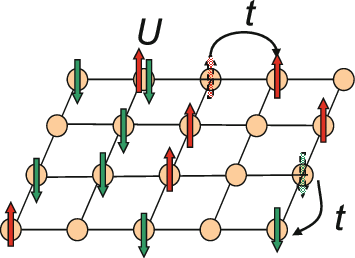
\includegraphics[width=0.8\linewidth]{pic2}
		\caption{\cite{Hubbard}}
		\label{fig:pic2}
	\end{subfigure}
	\begin{subfigure}{.5 \textwidth}
		\centering
		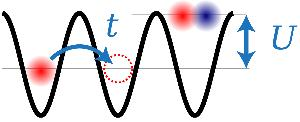
\includegraphics[width=0.8\linewidth]{pic1}
		\caption{\cite{Hubbard2}}
		\label{fig:pic1}
	\end{subfigure}
	\caption[Illustration of the Hubbard model]{(a): Twodimensional square lattice, orange points indicating atoms with one free orbital each and lattice lines indicating the permitted hops of the electrons. \\(b): Potential of a onedimensional lattice; here t denotes the kinetic energy of an electron when hopping to a neighboring lattice site (red and blue points) and U denotes the potential energy of two repulsing atoms of opposite spin.}
	\label{HubbardFigs}
\end{figure}
Figure \ref{fig:pic2} shows the lattice for a 2D material schematically. The onsite Coulomb repulsion is a feature that distinguishes the Hubbard model from most other models and enables it for instance to describe the transition from a metal to an insulator in certain materials. The Hamilton operator of the Hubbard model reads
\begin{equation}\label{Hubbard_original}
H = \sum_{i,j}\sum_{\sigma}T_{ij} c_{i\sigma}^\dag c_{j\sigma} + \frac{I}{2} \sum_{i}n_{i\uparrow}n_{i\downarrow} - \frac{I}{2}Nn^2
\end{equation}
where $ c^\dag $,  $ c $ and $ n = c^\dag c $ denote the creation operator, annihilation operator and occupation number operator respectively. Hopping from one lattice to another therefore corresponds to annihilating a particle at the intial lattice site and creating one at the final site. The Parameter I represents the potential energy of the Coulomb repulsion. The matrix element $ T_{ij} $ represents the kinetic energy when hopping from lattice site $i$ to lattice site $j$ and would in general depends on the orbital overlap of both sites, but an aditional assumption is made for the particles to only be able to hop to neighboring lattice sites.  That means for a homogeneous lattice $ T_{ij} \approx -t\delta_{\langle ij \rangle} $. This assumption simplifies the matrix a lot. Also writing  $ U = \frac{I}{2} $ and omitting the constant yields the simpler form of the Hamiltonian
\begin{equation}\label{Hubbard_standard}
H = \underbrace{-t\sum_{< i,j>,\sigma}\left( c_{i\sigma}^\dag c_{j\sigma} + c_{j\sigma}^\dag c_{i\sigma}\right)}_{\substack{H_0}}  + \underbrace{U \sum_{i}n_{i\uparrow}n_{i\downarrow}}_{\substack{H_I}}
\end{equation}
A pictorial representation of the meaning of the parameters $ t $ and $ U $ is illustrated in \ref{fig:pic1} with $t$ being a tunneling energy and $U$ being the potential energy of two particles on the same site. 
$ H_I $ defines the Coulomb part of the Hamiltonian and $H_0$ the hopping part.
%The hopping part of the Hamiltonian $H_0$ can be diagonalized by a Fouriertransformation to momentum space 
%\begin{equation}\label{Hubbard_momentum}
%H = \sum_{\boldsymbol{k} \sigma} \epsilon_{\boldsymbol{k}} c_{\boldsymbol{k}\sigma}^\dag c_{\boldsymbol{k}\sigma}\\
%\end{equation}
%$ \epsilon_{\boldsymbol{k}} $ denotes the dispersion relation of the electrons. The creation and annihilation are not acting on different lattice sites anymore, but on electrons with momentum $ \boldsymbol{k} $. They can be calculated as Wannierfunctions of the local operators
%\begin{equation}\label{Wannier}
%\psi_{\boldsymbol{k}} \left( \boldsymbol{x}\right) = \frac{1}{\sqrt{N}}\sum_{j} e^{i\boldsymbol{k}\boldsymbol{R}_j} \phi(\boldsymbol{x}-\boldsymbol{R}_j)
%\end{equation} 
%\begin{equation}\label{c_momentum}
%c_{\boldsymbol{k}\sigma} = \frac{1}{\sqrt{N}}\sum_{j} e^{i\boldsymbol{k}\boldsymbol{R}_j} c_{j\sigma}, \qquad c_{\boldsymbol{k}\sigma}^\dagger = \frac{1}{\sqrt{N}}\sum_{j} e^{-i\boldsymbol{k}\boldsymbol{R}_j} c_{j\sigma}^\dagger
%\end{equation}  
%Inserting this in \eqref{Hubbard_momentum} gives along with \eqref{Hubbard_original} the following expression for $ T_{ij} $ 
%\begin{equation}\label{T}
%T_{jl} = \frac{1}{N} \sum_{\boldsymbol{k}}\epsilon_{\boldsymbol{k}} e^{i\boldsymbol{k}\left( \boldsymbol{R}_j - \boldsymbol{R}_l\right) }
%\end{equation}

\subsection{Symmetries of the Hamiltonian}
If one considers both parts of the Hamiltonian diagonalization is not so easy. But one could in principle exploit the symmetries of the system to diagonalize it exactly. From the above defintion \eqref{Hubbard_standard} it becomes clear that the total particle number $ \hat{N} $ as well as the total spin $ \hat{S}^2 $ and its z-component $ \hat{S}_z $ are conserved quantities. This means that in a suitable basis the matrix will decouple into smaller block matrices along the diagonal. This enables one to look only on the block of most interest which in our case is the half-filled case. \\


Another symmetry is translational invariance. When considering a lattice with periodic boundary conditions it is obvious that translating all electrons by the same lattice vector, the observable quantities will not change, since the Hamilton operator does not depend on the absolute position of an electron. This implies that some states in the basis become the same when acting with a translation operator and are therefore equivalent.\\

\subsection{Finding the ground state analytically}
Finding the ground state energy is done in the next section for the 2 site model by explicit diagonalization. But this procedure becomes too time- and storage expensive for bigger lattices. For infinitely large lattices, which comes close to the case of a real material, the solution will converge to the following analytical solution
\begin{equation}\label{analytisch}
E_0(U)=-4L\int_{0}^{\infty}\frac{J_0(\omega)J_1(\omega)}{\omega\left( 1+\exp\left( \omega\frac{U}{2}\right) \right) }d\omega
\end{equation}\cite{lieb}
Here $ L $ denotes the number of lattice sites and $ J_n(\omega) $ is the Besselfunction of first kind.
\newline